\documentclass[conference,a4paper]{ieeetran}

\usepackage[latin1]{inputenc}
\usepackage{subeqnarray}
\usepackage{amsfonts}
\usepackage{amsmath}
\usepackage{amssymb}
\usepackage{graphicx}
\usepackage{color}
\usepackage{tikz}
\usepackage{tikz-qtree}
\usepackage{csquotes}
\usepackage{indentfirst}
\usepackage{upgreek}
\usepackage{forest}
\usepackage{hyperref}
\usepackage{pbox}
\usepackage{hhline}
\usepackage{datetime}
\usepackage{subcaption}
\usepackage{slashbox}
\usepackage[]{algorithm2e}
\usetikzlibrary{trees}
\usetikzlibrary{babel}
\usetikzlibrary{arrows,automata,positioning}

\usepackage[
    % maxbibnames=9,
    % maxnames=2,
    style=ieee,
    % citestyle=mla,
    backend=bibtex]
{biblatex}

\bibliography{biblio.bib}

\parskip 1mm
\arraycolsep 0.5mm
\newtheorem{theorem}{Theorem}
\newcommand{\sign}{\mathrm{sign}}
\newcommand{\sat}{\mathrm{sat}}

\newcommand*{\TitleFont}{%
      \usefont{\encodingdefault}{\rmdefault}{b}{n}%
      \fontsize{20}{24}%
      \selectfont}

\DeclareMathOperator*{\argminA}{arg\,min} % Jan Hlavacek

\newcommand{\argminD}{\arg\!\min} % AlfC

\title{\TitleFont{Phylogeny of JPEG images by ancestors estimation using missing markers on image pairs}}

% \author{\authorblockN{No� Le Philippe\authorrefmark{1}, William Puech\authorrefmark{1} and Christophe Fiorio\authorrefmark{1} }
% \authorblockA{\authorrefmark{1} LIRMM\\
% e-mail: noe.lephilippe@lirmm.fr, william.puech@lirmm.fr, fiorio@lirmm.fr}}


\author{\authorblockN{No� Le Philippe\authorrefmark{1}, William Puech \authorrefmark{1} and Christophe Fiorio\authorrefmark{1}}
\authorblockA{
\authorrefmark{1} LIRMM Laboratory, UMR 5506 \\
CNRS, University of Montpellier \\
Montpellier, France \\ 
e-mail: \{noe.lephilippe, william.puech, christophe.fiorio\}@lirmm.fr \\}}

\begin{document}
\maketitle
\begin{abstract}
 Nowadays it is extremely easy to tamper images and share them thanks to social media. Identifying the transformation history is mandatory to be able to trust any of those images. We address this problem using image phylogeny trees, where the root is the image the less tampered with and as every generation is obtainend from the transformation of its parents, the leaves are the most transformed images. Our method for image phylegeny trees reconstruction is based on a binary decision between two images using JPEG compression artifacts. Experimentals results show that in the case of no missing data, the reconstruction is very accurate.
\end{abstract}

\begin{keywords}
    Image phylogeny, JPEG compression, Social networks, Image phylogeny tree, near-duplicates
\end{keywords}

\section{Introduction}
It has never been so easy to share ideas and image content thanks to social networks. Every time content is shared however, its information can be altered, often not on purpose, as an image being recompressed to fit low bandwith networks would. But not always, there can also be malicious alteration that aim to modify the content meaning. To trust an image, it is mandatory to be able to tell whether content has been tampered with.

After every transformation, a new image is created. This new image is called a near-duplicate of its parent if, as defined by Joly \textit{et al.} \autocite{joly2007content}, it is a transformed version of a document that remains recognizable. It is formally defined as follows: $I_{n+1} = T(I_{n}), T \in \mathcal{T}$ where $I_{n}$ is the parent image at generation $n$, $I_{n+1}$ is the image at the next generation $n+1$, the child image, and $\mathcal{T}$ is a set of tolerated transformations, $I_{n+1}$ are $I_{n}$ near-duplicate images. The set $\mathcal{T}$ can contain any transformations, for instance, $\mathcal{T} = $ \textit{\{resampling, cropping, affine warping, color changing, lossy compression\}}. Authors used the words ``tolerated transformation'', their meaning is twofold. It limits the transformations to those present in the set $\mathcal{T}$ and sets an arbitrary limit to the strength of any given transformation. For example an image cropped by more than 20\% can be considered as a new image and not a near-duplicate.

In this paper, our goal is to identify the parent-child relationships in a set of near-duplicate images and extract the phylogeny of such relationships. The phylogeny is represented by a tree. The root is most likely the original image, or as close as possible to the original, unprocessed image. The leaves, on the other end of the spectrum, are the one most tampered with. We limit ourselves to the study of $\mathcal{T} = $ \textit{\{JPEG compression\}}, and specifically when the child image quality factor is smaller than its parent to focus on two main fields: image phylogeny, and forensics and multiple JPEG compression detection.

Most state of the art methods for image phylogeny tree estimation \autocites{dias2010first, dias2012image, 7018370, 7472039} have a two step method. First, they compute a dissimilarity matrix, an assymetric matrix, using a dissimilarity function. The dissimilarity function, given Equation \ref{eqn:dissimilarity}, is a function that, given two images, returns small values for similar images.

\begin{equation}
  d(I_{m},I_{n}) = \underset{T_{\overrightarrow{\beta}}}{min}\left | I_{n} - T_{\overrightarrow{\beta}}(I_{m}) \right |_{comparison\ method},
  \label{eqn:dissimilarity}
\end{equation}

where $I_{m}$ and $I_{n}$ are the images being compared, $T_{\overrightarrow{\beta}} \in \mathcal{T}$ is the transformation being estimated and $\overrightarrow{\beta}$ is a vector of all possible parameters of $T$. For JPEG compression, $\overrightarrow{\beta} = \{1..100\}$. The tree is then constructed using minimum spanning tree algorithms on the dissimilarity matrix.

% First they compute a dissimilarity matrix, an asymmetric matrix of distances between image pairs, and then compute a tree from this dissimilarity matrix. The dissimilarity matrix is built with a dissimilarity function, a function that yields small values for similar images. The tree is then constructed using minimum spanning trees algorithms. 
% Even the best tree reconstruction algorithm cannot return a good tree when the dissimilarity matrix was poorly estimated. Conversely, a bad tree reconstruction algorithm will not return a good tree.

JPEG compression, and in particular the detection of double JPEG compression, with the same quantization table \autocite{huang2010detecting} or not \autocite{lukavs2003estimation}, or with aligned grid or not \autocite{bianchi2012detection} has been largely studied. The detection is however often limited to at most two or three compressions and unless $Q_f = 100$ \autocite{CarneinSB2016TelltaleWatermarks}, we are not able to estimate the number of compressions the image underwent. In an image phylogeny tree, where JPEG compression is the only tolerated transformation, there will be a lot more than two compressions and traditionnal methods will not be very effective. The problem is rather to know whether an image is the result of the compression of another one, and which one, and whether an image has been compressed more times than another one.

Section \ref{sec:method} presents our method, the theorems and definitions we introduced, the ancestor estimation and the tree reconstruction. Section \ref{sec:results} shows our results and we discuss how and why we obtained them and finally section \ref{sec:conclusion} concludes our work and opens a few perspectives.
\section{Method}
\label{sec:method}
In this section, we present a new approach to build an image phylogeny tree from a set of near-duplicate images. Unlike state of the art methods that mainly focus on complex algorithm that try their best to approximate the tree from a dissimilarity matrix, we try to take a binary decision between two images: ``Can this image be an ancestor of that other one?''. It allows us to focus more on the images themselves and their characteristics and to have a simple tree reconstruction algorithm. Figure \ref{fig:schema} shows the diagram of our method.

\begin{figure}[!ht]
  \centering
  \scalebox{0.58}{
    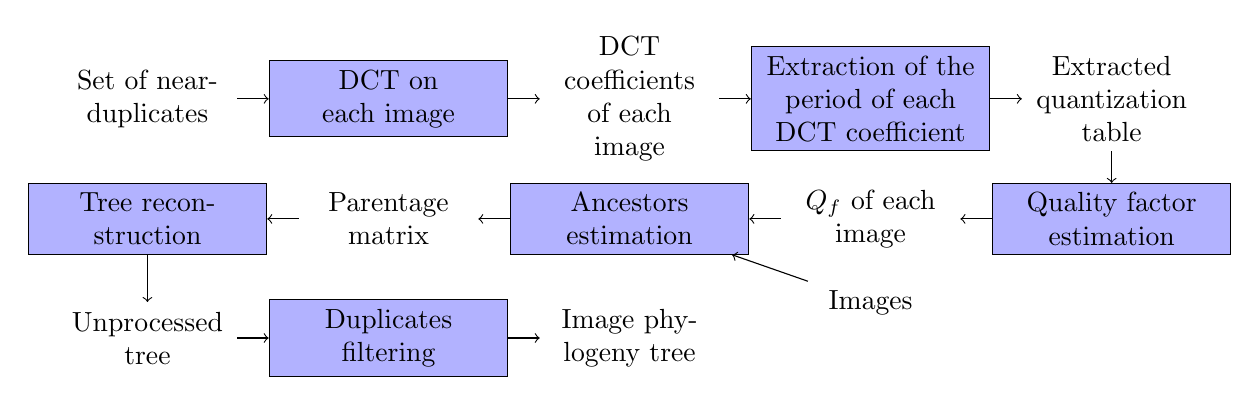
\begin{tikzpicture}[auto,node distance=2.1cm]

      \tikzstyle{every state}=[shape=rectangle,minimum width=1.1in,text width=1.1in, align=center,fill=blue!30]
      % \tikzstyle{every data}=[shape=circle,minimum width=1.3in,text width=1.3in, align=center,fill=blue!30]

      \node[draw=none,fill=none,minimum width=0.8in,text width=0.8in, align=center] (A) {Set of near-duplicates};
      \node[state] (B) [right=0.4cm of A] {DCT on each image};

      \node[draw=none,fill=none,minimum width=0.8in,text width=0.8in, align=center, right=0.4cm of B] (C) {DCT coefficients of each image};
      \node[state] (D) [right=0.4cm of C] {Extraction of the period of each DCT coefficient};

      \node[draw=none,fill=none,minimum width=0.8in,text width=0.8in, align=center, right=0.4cm of D] (E) {Extracted quantization table};
      \node[state] (F) [below=0.4cm of E] {Quality factor estimation};

      \node[draw=none,fill=none,minimum width=0.8in,text width=0.8in, align=center, left=0.4cm of F] (G) {$Q_f$ of each image};
      \node[draw=none,fill=none,minimum width=0.8in,text width=0.8in, align=center, below=0.3cm of G] (H) {Images};
      \node[state] (I) [left=0.4cm of G] {Ancestors estimation};

      \node[draw=none,fill=none,minimum width=0.8in,text width=0.8in, align=center, left=0.4cm of I] (J) {Parentage matrix};
      \node[state] (K) [left=0.4cm of J] {Tree reconstruction};

      \node[draw=none,fill=none,minimum width=0.8in,text width=0.8in, align=center, below=0.6cm of K] (L) {Unprocessed tree};
      \node[state] (M) [right=0.4cm of L] {Duplicates filtering};
      
      \node[draw=none,fill=none,minimum width=0.8in,text width=0.8in, align=center, right=0.4 of M] (N) {Image phylogeny tree};

      \path [->] (A) edge node[left] {} (B);
      \path [->] (B) edge node[left] {} (C);      
      \path [->] (C) edge node[left] {} (D);      
      \path [->] (D) edge node[] {} (E);      
      \path [->] (E) edge node[right] {} (F);      
      \path [->] (F) edge node[right] {} (G);      
      \path [->] (G) edge node[left] {} (I); 
      \path [->] (H) edge node[left] {} (I);
      \path [->] (I) edge node[left] {} (J);
      \path [->] (J) edge node[left] {} (K);
      \path [->] (K) edge node[left] {} (L);
      \path [->] (L) edge node[left] {} (M);
      \path [->] (M) edge node[left] {} (N);
    \end{tikzpicture}}
  \caption{Diagram of our method.}
  \label{fig:schema}
\end{figure}

In this section, we will first present the theorem we based designed our method on, then we explain how we extract the period of each DCT coefficient to extract a quantization table. We also explain how we compute the quality factor of an image and estimate the ancestors. We then present our tree reconstruction algorithm that will eventually output an image phylogeny tree.

\subsection{Theorems}
For every image pair in the set, we take a binary decision that will allow us to build a parentage matrix. We try to decide whether an image is an ancestor of another one. We set up a framework to solve this problem.

\newtheorem{marqueur}{Definition}
\newtheorem{fonction}{Definition}

\begin{marqueur}
  A marker is a local or global feature extracted from the image. This marker shows that a particular transformation was applied to the image. This marker is passed on the image children, and will be used to prove that an image is not an ancestor of another one. For instance a grayscale image cannot be an ancestor of a color image because the ``color'' marker is missing.
\end{marqueur}

\begin{fonction}
Let $f(I_{m},I_{n})$ be a function that for every image pair $(I_{m}, I_{n})$ detects every time there is one a marker visible in the image $I_m$ and not in its potential child $I_n$, thus proving that $I_m$ is not an ancestor of $I_n$. This function is called a negation function. This is an abstract function, and that is where lies the difficulty.
\end{fonction}

\newtheorem{parentage}{Theorem}
\begin{parentage}
For all image pair ($I_{m}$, $I_{n}$) in a set of near-duplicate images, if there is no marker proving that $I_m$ is not an ancestor of $I_n$ then there is a parent-child relationship between $I_{m}$ and $I_{n}$, $I_{m}$ $\to$ $I_{n}$, with $m < n$.
\end{parentage}

\begin{proof}
  If $f(I_{m},I_{n})$ cannot find a marker that proves that $I_m$ is not an ancestor of $I_n$ then this marker does not exist, thus $I_{m}$ is an ancestor of $I_{n}$, with $m < n$.
\end{proof}


\subsection{Quality factor estimation}
\label{subsec:qfestimation}
We work with images that underwent at least one JPEG compression. These images, traveling through social networks, may have had their format changed, and converted to raw format for instance. The quality factor $Q_f$ of the last JPEG compression, mandatory for our method, is then lost. We propose to estimate the quality factor of images that did not undergo any lossless compression other than JPEG.

\subsubsection{Quantization table extraction}
when a signal is quantized, its values gather around multiples of the quantization step. The gap between these values, the period, is what we are going to compute for the first 35 DCT coefficients of the image (in zigzag order). We only use the first 35 because further coefficients are often too quantized and have many null values to be of any use: we may badly estimate their period, and hinder the table extraction process. To get these periods, we compute the auto-correlation of a signal, as shown Fig. \ref{fig:autocorrelation}. We only keep the first few peaks above a threshold. It allows us to filter out the noise and not have missing peaks because of the threshold, as we would have Fig. \ref{fig:autocorrelation} with peaks alternating above and below the threshold. We repeat this process for every DCT coefficient selected, it outputs a partial quantization table, named $\widehat{q}(u,v)$, with $u, v \in \{0,...,7\}$. Next we compute $Q_f$ from $\widehat{q}(u,v)$.

\begin{figure}[!ht]
\centering
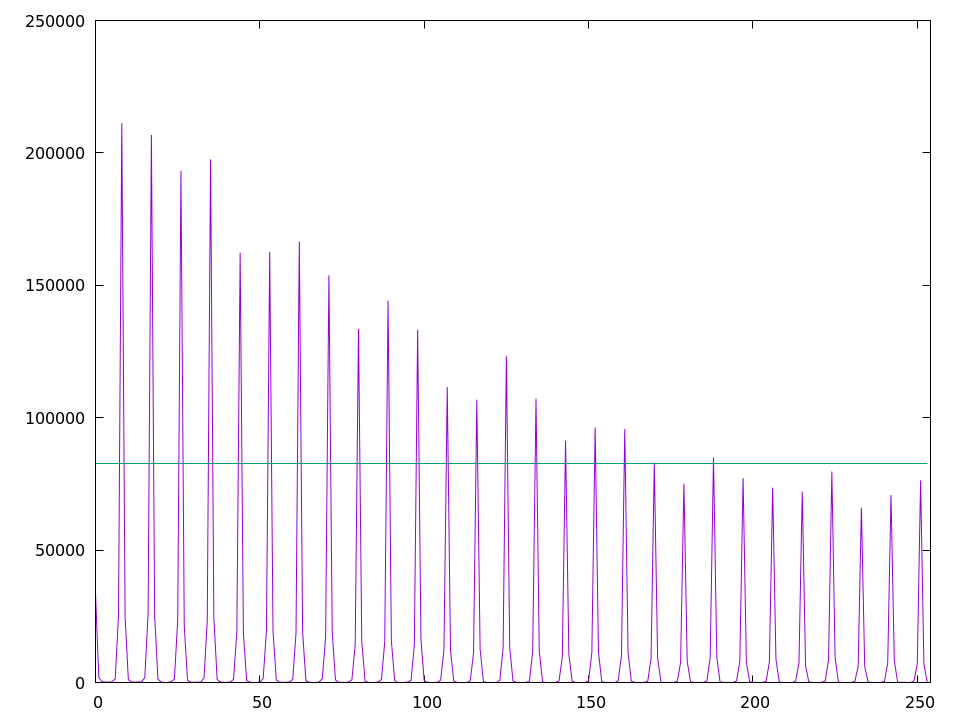
\includegraphics[width=7cm]{autocorrelation_filtered}
\caption{Auto-correlation of the DC coefficients and the threshold in green.}
\label{fig:autocorrelation}
\end{figure}

\subsubsection{Quality factor estimation}
we use a two step method to estimate the quality factor $Q_f$ from $\widehat{q}(u,v)$. The first step is called the primary estimation, where we check against every single quantization table from $Q_f = 1$ to $Q_f = 100$ which one is closest, the second step, the secondary estimation, uses equations \ref{eqn:jpeg_1} and \ref{eqn:jpeg_2} from the JPEG standard and the $Q_f$ obtained from the primary estimation to return a more accurate quality factor.

% we have two choices to compute the quality factor from $\widehat{q}(u,v)$. We can either check against every single quantization table from $Q_f = 1$ to $Q_f = 100$ which one is closest or use equations \ref{eqn:jpeg_1} and \ref{eqn:jpeg_2} from the JPEG standard:

\begin{equation}
\begin{split}
 if\ \ \  Q_f < 50\ \ \ \  Q_s = 5000 / Q_f \\
 else \ \ Q_s = 200 - (Q_f \times 2)\ \ \ \ \ \ 
\end{split}
\label{eqn:jpeg_1}
\end{equation}

\begin{equation}
\begin{split}
  q(u,v) = \frac{(q_{50}(u,v) \times Q_s) - 50}{100} \\ 
  with \ 1 \leq q(u,v) \leq 255
\end{split}
  \label{eqn:jpeg_2}
\end{equation}

where $q_{50}$ is the reference JPEG quantization table for $Q_f = 50$.
% $Q_f = \argminA_n D_{euc}(\widehat{q}(u,v), q_n(u,v))$

During the primariy estimation, the $Q_f$ is $n$ the index of the minimal distance between $q_n(u,v)$ and $\widehat{q}(u,v),\ n\in \{1..100\}$. It is the most similar quantization table, the most probable table used for compression. The primary $Q_f$ is then used to select the adequate equation for $Q_s$ in Equation \ref{eqn:jpeg_1}. Thus, a $Q_f*$ is computed for each coefficient in the partial quantization table $\widehat{q}(u,v)$. The actual $Q_f$ is the mean of all $Q_f*$.  We should add that even if after the primary estimation, $Q_f$ is incorrectly estimated above 50, the difference between both cases in equation \ref{eqn:jpeg_1} is small for values of $Q_f$ close to 50. The estimated $Q_f$ is not always exactly the real $Q_f$ anyway, we address this problem in the ancestor estimation.
% Using Equations \ref{eqn:jpeg_1} and \ref{eqn:jpeg_2}, even if it is light and fast, has one main issue: it cannot compute $Q_f$. It is possible to get $Q_s$ from Equation \ref{eqn:jpeg_2}, but it is not possible to get $Q_f$ from $Q_s$ in equation \ref{eqn:jpeg_1} without knowing whether $Q_s$ is greater than 50. 

% We chose to use both methods. We get a first estimation of $Q_f$ by finding which table from $q_n(u,v)$ is most similar to $\widehat{q}(u,v)$, we call this step primary estimation. With this primary estimation of $Q_f$, we refine our estimation by using equations \ref{eqn:jpeg_1} and \ref{eqn:jpeg_2}. Thus, a $Q_f*$ is computed for each coefficient in the partial quantization table $\widehat{q}(u,v)$. The actual $Q_f$ is the mean of all $Q_f*$. This step is called secondary estimation. We should add that even if after the primary estimation, $Q_f$ is incorrectly estimated above 50, the difference between both cases in equation \ref{eqn:jpeg_1} is small for values of $Q_f$ close to 50. The estimated $Q_f$ is not always exactly the real $Q_f$ anyway, we address this problem in the ancestor estimation.

\subsection{Ancestors estimation}
The quality factor $Q_f$ used to compress the image is mandatory to estimate the ancestors. Not only is it a very effective marker to filter out images that cannot be ancestors, the quality factor also allows us to normalize images to better compare them. 

We assume that JPEG compression is a deterministic operation. That is, for the same implementation the same input will always output the same result. This implies that all compressions of the same image will be identical, for any number of compression the image underwent beforehand. As explained before, we limit ourselves to JPEG compression, it means that to obtain a child image from its parent, the parent was JPEG compressed. An ancestor is called the parent if it is one transformation away from its child, one compression away in our case.

From this, we can accurately estimate the parent: 

Let $I_m$ and $I_n$ be two images and $Q_{f_{m}}$ and $Q_{f_{n}}$ their quality factors, and $C(I,Q_f)$ a JPEG compression operator, with $I$ an image and $Q_f$ a quality factor.
\\

If $I_n = C(I_m, Q_{f_{n}})$, then $I_m$ is the parent of $I_n$.

As we stated section \ref{subsec:qfestimation}, our $Q_f$ is not always the right $Q_f$, but can be too big or too small. We solve that testing $Q_f$ and its neighbors as compression candidates until a ancestor is found. The running time of our algorithm is closely related with the accuracy of the estimation of our $Q_f$'s. This method, even if it yields excellent results, can only find the direct parent and not further ancestors. It is indeed not easy to take a binary decision when the bounds of the values changes so much with the input data.

\subsection{Tree reconstruction}
The ancestor estimation process output a binary matrix of size $n\times n,\ n$ being the number of images in the set. This matrix is called a parentage matrix. A 1 value at index $(i, j)$ in this matrix means that image $I_i$ is an ancestor of image $I_j$. A 0 value tells us they are not related. Figure \ref{fig:tree} shows an example of a tree with its parentage matrix.

\begin{figure}[htbp]
  \begin{subfigure}{.25\textwidth}
    \centering
    % 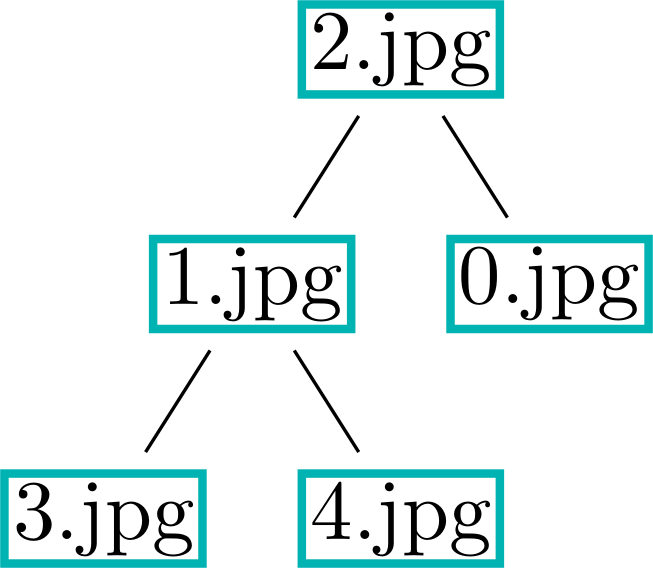
\includegraphics[width=.7\linewidth]{algo_tree}
    \scalebox{1.1}{
      \begin{forest}
        [\href{run:2}{2.jpg}[\href{run:1}{1.jpg}[\href{run:3}{3.jpg}][\href{run:4}{4.jpg}]][\href{run:0}{0.jpg}]]
      \end{forest}}
    \caption{Phylogeny tree}
    \label{algo_tree}
  \end{subfigure}%
  \begin{subfigure}{.25\textwidth}
    \centering
    \begin{tabular}{|r||c|c|c|c|c|}
      \hline
      - & $I_{0}$ & $I_{1}$ & $I_{2}$ & $I_{3}$ & $I_{4}$ \\ \hhline{|=::=|=|=|=|=|}
      $I_{0}$ & - & 0 & 0 & 0 & 0 \\ \hline
      $I_{1}$ & 0 & - & 0 & 1 & 1 \\ \hline
      $I_{2}$ & 1 & 1 & - & 1 & 1 \\ \hline
      $I_{3}$ & 0 & 0 & 0 & - & 0 \\ \hline
      $I_{4}$ & 0 & 0 & 0 & 0 & - \\ \hline
    \end{tabular} 
    \caption{Parentage matrix}
    \label{parentage_matrix}
  \end{subfigure}
  \caption{An example of a phylogeny tree and its parentage matrix.}
  \label{fig:tree}
\end{figure}

From this example, we can notice several things. A column with only 0 values does not have any ancestor, it is then the root of the tree, which, by definition, does not have ancestors. A row with only 0 values is the parent of no one: it is a leaf. We can generalize and say that the less a column has 0 values, the less ancestors it has, the closest it is to the root. Algorithm \ref{algo_} presents our tree reconstruction algorithm.

\begin{algorithm}[]
  \LinesNumbered
  \KwData{M a $n\times n$ parentage matrix}
  \KwResult{the root of the tree}
  \BlankLine
  $nextRoot \leftarrow$ row with min sum of elements\;
  $treeRoot \leftarrow nextRoot$\;
  \BlankLine

  \ForAll{rows row of M}{
    $root \leftarrow nextRoot$\;
    mark $root$ as done\;
    \BlankLine
    \For{$i\leftarrow 0$ \KwTo n}{
      $row[i] \leftarrow 0$\;
      \If{sum of elements of row = 0} {
        add $i$ as child of $root$\;
      }
      \If{row has the smallest sum of elements and is not marked as done} {
        $nextRoot \leftarrow i$\;
      }
    }
  }
  \KwRet treeRoot
\caption{Tree reconstruction algorithm.}
\label{algo_}
\end{algorithm}

At each iteration, an image is selected as the root (lines 1 and 11) and named $root$. $root$ is removed (line 7) from the ancestors of the other images. If these other images do not have any ancestor (line 8), it means that $root$ was the direct parent of the image being processed. This image is added as a child of $root$ (line 9). Line 5 prevents images from being a potential root twice. This algorithm runs in $O(n^2)$. It has two nested loops and if the sums are computed once at the beginning and updated every time a parent is removed, there is no extra loop increasing complexity.

\section{Experiments and results}
\label{sec:results}
In this section, we presents the results we obtained with our method. We start by describing how our datasets were generated and then explain our results and how and why they were obtained.

\subsection{Dataset generation}
We created three datasets, one with trees with 15 images, another one with 25 images and a last one with 50 images. It allows us to see how things like the distance to the root or the number of compressions affect our tree estimation method.

From a seed images (never lossy compressed), a first image is compressed with $85 < Q_f < 99$, it is the root image. This image is added to the images pool. While the number of images in the pool is smaller than the desired number, an image is randomly chosen in the pool, compressed with $Q_{f_{parent}} - 15 < Q_{f_{child}} < Q_{f_{parent}} - 1$ and added to the pool. The quality factor cannot be smaller than 30, further than that, the image is both too deteriorated and does not contain meaningful information and not a realistic use case on social networks. We used the six base images of BOWS 2 \autocite{bows}, where each image was used to create 15 trees for each tree size, a total of 90 trees per dataset, or 8100 images.

\subsection{Details on a tree}
%% unfold algorithms on a dataset
Before giving the results of our method on our datasets, we unfold our algorithms on a 15 images tree as an example for the reader to better visualize how our algorithms work. We use one image of this dataset to show how its quality factor is estimated and then expand to the rest of the tree.
The chosen image has the following compression history�: $H_{Q_{f}} = \{86, 85, 73\}$. A partial quantization table $\widehat{q}(u,v)$ is computed using auto-correlation and peak detection techniques. The table $\widehat{q}(u,v)$ for this image is available Fig. \ref{periods1}. The next step is the primary estimation, where $\widehat{q}(u,v)$ is checked against every quantization table from $Q_f = 1$ to $Q_f = 100$. Figure \ref{fig:distances} shows the distance between $\widehat{q}(u,v)$ and every other quantization tables. The primary estimation returns $Q_f = 71$, the quantization table of $Q_f = 71$ is available Fig.~\ref{periods2} for comparison as well as the table of $Q_f = 73$ Fig.~\ref{periods3}, the actual quality factor. A negative value in $\widehat{q}(u,v)$ means that no peak was detected and that no period was estimated, a 0 value means that the coefficient outside of the 35 coefficients range.

\begin{figure}
  \begin{subfigure}{.5\textwidth}
    \centering
    \begin{tabular}{|c|c|c|c|c|c|c|c|}
      \hline
      9 & 6 & 5 & 9 & 13 & 22 & 22 & 31 \\ \hline    
      6 & 6 & 8 & 10 & 14 & 16 & 28 & 0 \\ \hline
      8 & 7 & 9 & 13 & 20 & -1 & 0 & 0 \\ \hline
      8 & 9 & 12 & 19 & -1 & -1 & 0 & 0 \\ \hline
      10 & 12 & -1 & 31 & 30 & 0 & 0 & 0 \\ \hline
      12 & 13 & 28 & 30 & 0 & 0 & 0 & 0 \\ \hline
    \end{tabular}
    \caption{Quantization table returned by periods estimation, $\widehat{q}(u,v)$.}
    \label{periods1}
  \end{subfigure}
 \vspace{5mm}

  \begin{subfigure}{.5\textwidth}
    \centering
    \begin{tabular}{|c|c|c|c|c|c|c|c|}
      \hline
      9 & 7 & 8 & 8 & 10 & 14 & 28 & 42 \\ \hline
      6 & 7 & 8 & 10 & 13 & 20 & 37 & 53 \\ \hline
      6 & 8 & 9 & 13 & 21 & 32 & 45 & 55 \\ \hline
      9 & 11 & 14 & 17 & 32 & 37 & 50 & 57 \\ \hline
      14 & 15 & 23 & 30 & 39 & 47 & 60 & 65 \\ \hline
      23 & 34 & 33 & 50 & 63 & 60 & 70 & 58 \\ \hline
    \end{tabular}
    \caption{Best quantization table found during the primary estimation where the distance between $\widehat{q}(u,v)$ and table(i) is minimal, $i = 71$.}
    \label{periods2}
  \end{subfigure}
\vspace{5mm}

 \begin{subfigure}{.5\textwidth}
    \centering
    \begin{tabular}{|c|c|c|c|c|c|c|c|}
      \hline
      9 & 6 & 8 & 8 & 10 & 13 & 26 & 39  \\ \hline
      6 & 6 & 7 & 9 & 12 & 19 & 35 & 50  \\ \hline
      5 & 8 & 9 & 12 & 20 & 30 & 42 & 51  \\ \hline
      9 & 10 & 13 & 16 & 30 & 35 & 47 & 53  \\ \hline
      13 & 14 & 22 & 28 & 37 & 44 & 56 & 60  \\ \hline
      22 & 31 & 31 & 47 & 59 & 56 & 65 & 54  \\ \hline
    \end{tabular}
    \caption{Quantization table of the actual $Q_f$, $i = 73$.}
    \label{periods3}
  \end{subfigure}
  \caption{Example of quantization tables used during the tree reconstruction.}
\end{figure}

\begin{figure}[!ht]
\centering
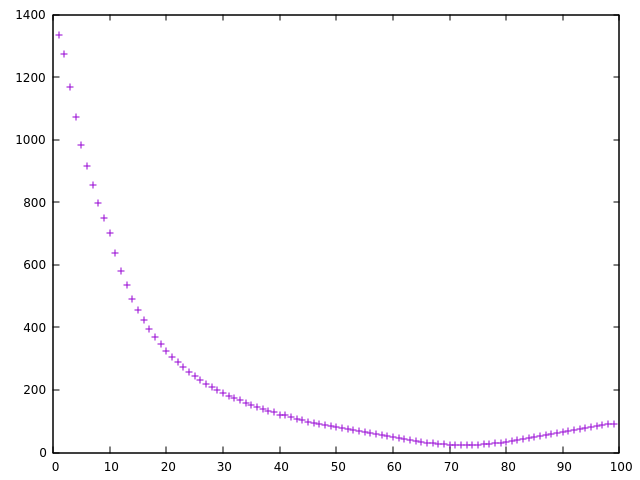
\includegraphics[width=7cm]{distances}
\caption{Distances between $\widehat{q}(u,v)$ and table(i).}
\label{fig:distances}
\end{figure}

All images in the set undergo the same process, followed by the secondary estimation. Table \ref{rough_fine} shows how the secondary estimation improves the primary estimation.
%primary estimation is improved by the secondary estimation. 
\begin{table*}
  \centering
  \begin{tabular}{|l||c|c|c|c|c|c|c|c|c|c|c|c|c|c|c|}
    \hline
    Image & $I_{0}$ & $I_{1}$ & $I_{2}$ & $I_{3}$ & $I_{4}$ & $I_{5}$ & $I_{6}$ & $I_{7}$ & $I_{8}$ & $I_{9}$ & $I_{10}$ & $I_{11}$ & $I_{12}$ & $I_{13}$ & $I_{14}$ \\ \hhline{|=::=|=|=|=|=|=|=|=|=|=|=|=|=|=|=|}
   
    \textbf{Primary}  & 71 & 81 & 71 & 58 & 78 & 46 & 61 & 85 & 81 & 79 & 65 & 74 & 84 & 71 & 74 \\ \hline
    \textbf{Secondary} & 71 & 81 & 71 & 58 & 78 & 46 & 61 & 87 & 82 & 80 & 65 & 74 & 85 & 71 & 75 \\ \hline
    \textbf{Actual value} & 73 & 81 & 71 & 57 & 79 & 44 & 62 & 86 & 82 & 80 & 65 & 74 & 85 & 71 & 75 \\ \hline
    % \textbf{Delta primaire} & -2 & 0 & 0 & 1 & -1 & 2 & -1 & -1 & -1 & -1 & -1 & 0 & -1 & 0 & -1 \\ \hline
    % \textbf{Delta secondaire} & -2 & 0 & 0 & 1 & -1 & 2 & -1 & 1 & 0 & 0 & 0 & 0 & 0 & 0 & 0 \\ \hline
  \end{tabular}

  \caption{Primary and secondary estimation of $Q_f$ for every image in the set.}
  \label{rough_fine}
\end{table*}
This secondary estimation is used to compress images to normalize and compare them. Table \ref{table:parentage_matrix} shows the parentage matrix returned by our algorithm. We can see that there is at most one 1 value per line, it means that only the parent was found and no other ancestor. Finally, Fig. \ref{fig:tree_reconstructed} shows both the original tree and the reconstructed one. The trees are identical, all ancestry relationships are correct.

\begin{table}
  \centering
  \scalebox{0.69}{
  \begin{tabular}{|c||c|c|c|c|c|c|c|c|c|c|c|c|c|c|c|}
    \hline
    - & $I_{0}$ & $I_{1}$ & $I_{2}$ & $I_{3}$ & $I_{4}$ & $I_{5}$ & $I_{6}$ & $I_{7}$ & $I_{8}$ & $I_{9}$ & $I_{10}$ & $I_{11}$ & $I_{12}$ & $I_{13}$ & $I_{14}$ \\ \hhline{|=::=|=|=|=|=|=|=|=|=|=|=|=|=|=|=|}
    $I_{0}$ & - & 0 & 0 & 0 & 0 & 0 & 0 & 0 & 0 & 0 & 0 & 0 & 1 & 0 & 0 \\ \hline 
    $I_{1}$ & 0 & - & 0 & 0 & 0 & 0 & 0 & 0 & 1 & 0 & 0 & 0 & 0 & 0 & 0 \\ \hline 
    $I_{2}$ & 0 & 0 & - & 0 & 0 & 0 & 0 & 0 & 0 & 0 & 0 & 0 & 1 & 0 & 0 \\ \hline 
    $I_{3}$ & 0 & 0 & 0 & - & 0 & 0 & 0 & 0 & 0 & 0 & 0 & 0 & 0 & 1 & 0 \\ \hline 
    $I_{4}$ & 0 & 0 & 0 & 0 & - & 0 & 0 & 0 & 0 & 0 & 0 & 0 & 1 & 0 & 0 \\ \hline 
    $I_{5}$ & 0 & 0 & 0 & 1 & 0 & - & 0 & 0 & 0 & 0 & 0 & 0 & 0 & 0 & 0 \\ \hline 
    $I_{6}$ & 0 & 0 & 0 & 0 & 0 & 0 & - & 0 & 0 & 0 & 1 & 0 & 0 & 0 & 0 \\ \hline 
    $I_{7}$ & 0 & 0 & 0 & 0 & 0 & 0 & 0 & - & 0 & 0 & 0 & 0 & 0 & 0 & 0 \\ \hline 
    $I_{8}$ & 0 & 0 & 0 & 0 & 0 & 0 & 0 & 1 & - & 0 & 0 & 0 & 0 & 0 & 0 \\ \hline 
    $I_{9}$ & 0 & 1 & 0 & 0 & 0 & 0 & 0 & 0 & 0 & - & 0 & 0 & 0 & 0 & 0 \\ \hline 
    $I_{10}$& 0 & 0 & 0 & 0 & 0 & 0 & 0 & 0 & 0 & 0 & - & 0 & 0 & 1 & 0 \\ \hline 
    $I_{11}$& 0 & 0 & 0 & 0 & 0 & 0 & 0 & 1 & 0 & 0 & 0 & - & 0 & 0 & 0 \\ \hline 
    $I_{12}$& 0 & 0 & 0 & 0 & 0 & 0 & 0 & 1 & 0 & 0 & 0 & 0 & - & 0 & 0 \\ \hline 
    $I_{13}$& 0 & 0 & 0 & 0 & 0 & 0 & 0 & 0 & 1 & 0 & 0 & 0 & 0 & - & 0 \\ \hline 
    $I_{14}$& 0 & 0 & 0 & 0 & 0 & 0 & 0 & 0 & 0 & 1 & 0 & 0 & 0 & 0 & - \\ \hline 

  \end{tabular}}
  \caption{Parentage matrix.}
  \label{table:parentage_matrix}
\end{table}

\begin{figure}[htpb]
  \begin{subfigure}{.5\textwidth}
    \centering
    \scalebox{0.7}{
      \begin{forest}
        [\href{run:7.jpg}{7.jpg}[\href{run:8.jpg}{8.jpg}[\href{run:13.jpg}{13.jpg}[\href{run:3.jpg}{3.jpg}[\href{run:5.jpg}{5.jpg}]][\href{run:10.jpg}{10.jpg}[\href{run:6.jpg}{6.jpg}]]][\href{run:1.jpg}{1.jpg}[\href{run:9.jpg}{9.jpg}[\href{run:14.jpg}{14.jpg}]]]][\href{run:12.jpg}{12.jpg}[\href{run:2.jpg}{2.jpg}][\href{run:4.jpg}{4.jpg}][\href{run:0.jpg}{0.jpg}]][\href{run:11.jpg}{11.jpg}]]
      \end{forest}}
    \caption{Original image phylogeny tree.}
  \end{subfigure}
  \begin{subfigure}{.5\textwidth}
    \centering
    \scalebox{0.7}{
      \begin{forest}
        [\href{run:7}{7.jpg}[\href{run:8}{8.jpg}[\href{run:1}{1.jpg}[\href{run:9}{9.jpg}[\href{run:14}{14.jpg}]]][\href{run:13}{13.jpg}[\href{run:3}{3.jpg}[\href{run:5}{5.jpg}]][\href{run:10}{10.jpg}[\href{run:6}{6.jpg}]]]][\href{run:11}{11.jpg}][\href{run:12}{12.jpg}[\href{run:0}{0.jpg}][\href{run:2}{2.jpg}][\href{run:4}{4.jpg}]]]
      \end{forest}}
    \caption{Reconstructed image phylogeny tree.}
    % \label{tree_example}
  \end{subfigure}
  \caption{Example of an image phylogeny tree and its reconstruction.}
  \label{fig:tree_reconstructed}
\end{figure}


\subsection{Experimental results}
We use seven metrics to measure our results, three metrics measuring the accuracy of the estimation of the quality factor, the four other, given by Dias \textit{et al.} \autocite{dias2010first} are %and available Fig. \ref{fig:metrics}.

\textbf{Root}: $R(IPT_{1}, IPT_{2}) = $
\scalebox{0.75}{%
  $\begin{cases}
    1 & if\ \texttt{Root(IPT}_{1}) = \texttt{Root(IPT}_{2}) \\
    0 & Otherwise
  \end{cases}$}

\textbf{Edges}: $E(IPT_{1}, IPT_{2}) = \frac{|E_{1} \cap E_{2}|} {n - 1}$

\textbf{Leaves}: $L(IPT_{1}, IPT_{2}) = \frac{|L_{1} \cap L_{2}|} {|L_{1} \cup L_{2}|}$

\textbf{Ancestry}:  $A(IPT_{1}, IPT_{2}) = \frac{|A_{1} \cap A_{2}|} {|A_{1} \cup A_{2}|}$

% \begin{figure}
% \renewcommand{\arraystretch}{2}
% \begin{tabular}{ll}
%   \textbf{Root} & $
%                   R(IPT_{1}, IPT_{2}) = $
%                   \scalebox{0.65}{%
%                   $
%                   \begin{cases}
%                     1 & if\ \texttt{Root(IPT}_{1}) = \texttt{Root(IPT}_{2}) \\
%                     0 & Otherwise
%                   \end{cases}
%                         $} \\
%   \textbf{Edges} & $E(IPT_{1}, IPT_{2}) = \frac{|E_{1} \cap E_{2}|} {n - 1}$ \\
%   \textbf{Leaves} & $L(IPT_{1}, IPT_{2}) = \frac{|L_{1} \cap L_{2}|} {|L_{1} \cup L_{2}|}$ \\
%   \textbf{Ancestry} & $A(IPT_{1}, IPT_{2}) = \frac{|A_{1} \cap A_{2}|} {|A_{1} \cup A_{2}|}$
% \end{tabular}
% \renewcommand{\arraystretch}{1.}
% \caption{Metrics for tree reconstruction evaluation.}
% \label{fig:metrics}
% \end{figure}

$Root$ is trivial and returns 1 if the roots of both trees are identical, $Edge$ measures the ratio of nodes which have the correct direct parent, $Leaves$ is the ratio of correct leaves and $Ancestry$ is the ratio of correct ancestors up to the root.

The three metrics used to measure the accuracy of the estimation of the quality factor is the estimation mean error, the mean error on all the $Q_f$'s on every image of the dataset. The mean overestimation and mean underestimation, which should be symmetrical, tells us whether our algorithm overestimates the $Q_f$'s, and when. Figures \ref{results} shows the results we got using our methods on the three datasets.

\begin{table}[htbp]
  \centering
  \scalebox{0.90}{
  \begin{tabular}{|l||c|c|c|c|c|}
    \hline
     \backslashbox{Metric}{Dataset}             & \textbf{15 images} & \textbf{25 images} & \textbf{50 images} \\ \hhline{|=::=|=|=|}
    \textbf{\pbox{2.6cm}{Mean estimation error of $Q_f$}} & 0.42 & 0.64 & 0.83 \\ \hline
    \textbf{\pbox{2.7cm}{Mean overestimation of $Q_f$}}      & 1.61  & 1.86  & 1.94  \\ \hline
    \textbf{\pbox{2.6cm}{Mean underestimation of  $Q_f$}}     & 1.07  & 2.12    & 6.68  \\ \hhline{|=::=|=|=|}
    \textbf{roots}                                              & 95.83 & 88.88 & 84.72 \\ \hline
    \textbf{edges}                                              & 99.70 & 99.24 & 98.97 \\ \hline
    \textbf{leaves}                                             & 99.59 & 99.15 & 98.74 \\ \hline
    \textbf{ancestry}                                           & 99.44 & 96.88 & 96.96 \\ \hline
  \end{tabular}} 
\caption{Results obtained from 8100 imgase, the first three metrics measure the accuracy of the estimation of $Q_f$, the others, which measure the quality of the tree reconstruction are given in percentage.}
\label{results}
\end{table}

We can see that the smaller the dataset, the better the results. We should add that the best score for the three first metrics is 0, when all $Q_f$ were correctly estimated, and the best score for the other is 100, when the two trees are identical.

The mean errors, even if they are below 1 for the three datasets, and are very good, get worse when the number of images increases, in particular the overestimation is pretty high for 50 images. This is due to too much noise on the DCT coefficients for images compressed a lot of times. We cannot properly estimated the period of such coefficients and therefore cannot properly estimate $Q_f$. When no peak is detected, our algorithm actually assumes that the image was not quantized, or compressed with a $Q_f$ very close to 100, since a signal not quantized will not show any peaks. A high number of compression is most likely to happen for 50 images, hence the worse results.

We assumed that JPEG compression was a deterministic operation. However, it appears not to be the case for small $Q_f$'s ($<$ 35) with a high number of compressions. It means that for some images, no parent can be found. We wanted to have a simple tree reconstruction algorithm, with only binary data, no other information is available during the reconstruction process. Thus, our algorithm cannot distinguish the root, which has no parent, and a problematic image, with no parents detected. The root is then chosen as the image with the smallest index. Again, this is most likely to occur on big datasets.

An other problem, which does not affect the root, but rather the rest of the tree, is block convergence, and image convergence, as shown by Lai and Bohme \autocite{lai2013block}. After a given number of compressions, an image can become identical to its parent, it then becomes impossible to tell which is which. This is caused by images with $Q_f = 30$, the lower bound of $Q_f$ during our generation. If an image with $Q_f = 30$ has a child, this child will also have $Q_f = 30$, and so recursively.

The results given Table \ref{results} are obtained on the whole dataset, where all images are available. Our method is very effective to estimate the phylogeny tree when all images are present, when there is always a direct parent. Since we cannot estimate other ancestors, we wanted to try our methods on the same dictates, with one image missing to see if the results were still good. Figure \ref{results_missing} shows the results.
\begin{table}
  \centering
  \scalebox{0.90}{
  \begin{tabular}{|l||c|c|c|c|c|}
    \hline
     \backslashbox{Metric}{Dataset}             & \textbf{15 images} & \textbf{25 images} & \textbf{50 images} \\ \hhline{|=::=|=|=|}
    \textbf{roots}                                                      & 69.60 & 33.33 & 49.01 \\ \hline
    \textbf{edges}                                                      & 88.86 & 92.40 & 95.07 \\ \hline
    \textbf{leaves}                                                     & 91.30 & 93.00 & 94.72 \\ \hline
    \textbf{ancestry}                                                   & 78.06 & 82.22 & 88.21 \\ \hline
  \end{tabular}}
\caption{Results with one image missing in each tree.}
\label{results_missing}
\end{table}
We can see that the root metric suffers the most from the image missing. Indeed, our tree reconstruction algorithm cannot differentiate an image with no parents (the root) and an image with no parents detected. The root of the tree is in this case almost randomly chosen. Figure \ref{fig:missing} shows how a tree with a missing node results can be obtained, giving an incorrect tree estimation. We actually have perfect subtrees, with the right parents, but we do not have the information on how to link those trees together.
\begin{figure}[htbp]
  \begin{subfigure}{.5\textwidth}
    \centering
    \begin{tikzpicture}
      \node[anchor=south west,inner sep=2] at (0,0) { 
        \begin{forest}
          [\href{run:7}{7.jpg}[\href{run:8}{8.jpg}[\href{run:1}{1.jpg}[\href{run:9}{9.jpg}[\href{run:14}{14.jpg}]]][\href{run:13}{13.jpg}[\href{run:3}{3.jpg}[\href{run:5}{5.jpg}]][\href{run:10}{10.jpg}[\href{run:6}{6.jpg}]]]][\href{run:11}{11.jpg}][\href{run:12}{12.jpg}[\href{run:0}{0.jpg}][\href{run:2}{2.jpg}][\href{run:4}{4.jpg}]]]
        \end{forest}};
      % \draw[red,ultra thick,rounded corners] (7.5,5.3) rectangle (9.4,6.2);
      \draw[red, ultra thick](0.8,2.5) -- (2.05,3.1);
      \draw[red, ultra thick](0.8,3.1) -- (2.05,2.5);
    \end{tikzpicture}
    \caption{Original tree with node 8 removed.}
  \end{subfigure}
  \begin{subfigure}{.5\textwidth}
    \centering
    \begin{tikzpicture}
      \node[anchor=south west,inner sep=2] at (0,0) { 
        \begin{forest}
          [\href{run:7}{7.jpg}[\href{run:11}{11.jpg}][\href{run:12}{12.jpg}[\href{run:0}{0.jpg}][\href{run:2}{2.jpg}][\href{run:4}{4.jpg}]]]
        \end{forest}
        \begin{forest}
          [\href{run:1}{1.jpg}[\href{run:9}{9.jpg}[\href{run:14}{14.jpg}]]]
        \end{forest}
        \begin{forest}
          [\href{run:13}{13.jpg}[\href{run:3}{3.jpg}[\href{run:5}{5.jpg}]][\href{run:10}{10.jpg}[\href{run:6}{6.jpg}]]]
        \end{forest}};
    \end{tikzpicture}
    \caption{Three subtrees that we do not know how to link.}
  \end{subfigure}

  \begin{subfigure}{.5\textwidth}
    \centering
    \begin{forest}
      [\href{run:1}{1.jpg}[\href{run:7}{7.jpg}[\href{run:11}{11.jpg}][\href{run:12}{12.jpg}[\href{run:0}{0.jpg}][\href{run:2}{2.jpg}][\href{run:4}{4.jpg}]]][\href{run:9}{9.jpg}[\href{run:14}{14.jpg}]][\href{run:13}{13.jpg}[\href{run:3}{3.jpg}[\href{run:5}{5.jpg}]][\href{run:10}{10.jpg}[\href{run:6}{6.jpg}]]]]
    \end{forest}
    \caption{Output of the tree reconstruction algorithm.}
    \label{fig:missing1}
  \end{subfigure}

  \caption{Example of a tree with a missing node and a reconstruction attempt.}
  \label{fig:missing}
\end{figure}

Even though our method was designed for grayscale images, we wanted to see if the luminance channel of a color image contained enough information for our method to estimate the tree. None of our algorithm were modified and we only gave color images instead of grayscale images as input. Table \ref{results_color} shows our results.
\begin{figure}[htbp]
  \centering
\scalebox{0.90}{
  \begin{tabular}{|l||c|c|c|c|c|}
    \hline
     \backslashbox{Metric}{Dataset}             & \textbf{15 images} & \textbf{25 images} & \textbf{50 images} \\ \hhline{|=::=|=|=|}
    \textbf{\pbox{2.6cm}{Mean estimation error of $Q_f$}}               & 1.15  & 1.29  & 1.42     \\ \hline
    \textbf{\pbox{2.7cm}{Mean overestimation of $Q_f$}}                 & 1.85  & 2.70  & 2.64  \\ \hline
    \textbf{\pbox{2.6cm}{Mean underestimation of  $Q_f$}}               & 2.97  & 3.79  & 4.94  \\ \hhline{|=::=|=|=|}
    \textbf{roots}                                                      & 93.94 & 81.82 & 87.88 \\ \hline
    \textbf{edges}                                                      & 99.35 & 98.61 & 99.38 \\ \hline
    \textbf{leaves}                                                     & 99.62 & 98.66 & 99.78 \\ \hline
    \textbf{ancestry}                                                   & 98.79 & 94.13 & 98.82 \\ \hline
  \end{tabular}}
\caption{Results table with color images.}
\label{results_color}
\end{figure}
The results are not very different from grayscale images, slightly worse, but not significantly so. The estimation of $Q_f$ is not as good, it is because of the rounding when going from RGB to YUV. We did not use any of the chrominance channel, the luminance channel seems to contain enough information and allows us to reliably estimate the tree.

\section{Conclusion}
\label{sec:conclusion}

"Sed ut perspiciatis unde omnis iste natus error sit voluptatem accusantium doloremque laudantium, totam rem aperiam, eaque ipsa quae ab illo inventore veritatis et quasi architecto beatae vitae dicta sunt explicabo. Nemo enim ipsam voluptatem quia voluptas sit aspernatur aut odit aut fugit, sed quia consequuntur magni dolores eos qui ratione voluptatem sequi nesciunt. Neque porro quisquam est, qui dolorem ipsum quia dolor sit amet, consectetur, adipisci velit, sed quia non numquam eius modi tempora incidunt ut labore et dolore magnam aliquam quaerat voluptatem. Ut enim ad minima veniam, quis nostrum exercitationem ullam corporis suscipit laboriosam, nisi ut aliquid ex ea commodi consequatur? Quis autem vel eum iure reprehenderit qui in ea voluptate velit esse quam nihil molestiae consequatur, vel illum qui dolorem eum fugiat quo voluptas nulla pariatur?"

\printbibliography

\end{document}
